\chapter[Professor G Ramachandran- My Guru]{Professor G Ramachandran- My Guru}\label{chap15}

As a student of M.Sc. in physics from 1977 to 79, I came to know Prof. G Ramachandran a year later, when four of us chose theoretical physics as our specialization. I very well remember those days of M.Sc when we used to watch our seniors, especially those who chose the same specialization, expecting some clues from them on how to tune ourselves for the course. I do not remember all of them except Dr. K N Nagendra (who unfortunately passed away a year before Prof. GR) and Dr. Govindaraj (I am not very sure of his exact name now). Of the two, Dr. Nagendra appeared to be much disciplined, while Dr. Govindaraj was on the other extreme, always appearing jovial and very social. I still remember some of the unique talents he exhibited in the Welcome and Farewell parties during that time. I say all this because that was a very important stage in our lives as students. Although we were already halfway through in achieving our goal to get an M.Sc. degree in Physics, a new dilemma started bothering us at the end of the first year and this was precisely regarding which specialization one should choose in the coming year. We had heard lectures by several good teachers. What is green in my memory even today are the classes handled by Professors K N Srinivasa Rao (KNS), K Gopala, P Venkataramaiah, H S Subramaniam, and A V Gopala Rao (AVG). I must confess, as many of my classmates also felt, that it was not so easy to follow Prof. K N Srinivasa Rao's teaching. Amid his lecturing, he would ask questions that would be so difficult to answer and our classmate M Ravindra, who got the first rank in B.Sc., used to steal the show by giving correct answers; he later joined ISRO. As I now remember, Prof. B Sanjeevaiah, the then Chairman of the Department, Professors D Krishnamurthy, H Sanjeevaiah, N Sreedhara Murthy, G Ramachandran, and Shantha Venkataraman had not taken classes in our first year and we often used to imagine how their classes would be. It so happened that only four of us got into Theoretical Physics spe- cialization citing different reasons at that time and against the warnings by some of our seniors that Theoretical Physics was the most difficult of the four available options. While Nuclear physics and Solid state physics enjoyed high popularity, Theoretical Physics was loaded with a heavily packed syllabus. Besides this, we also had to answer an additional paper in the theory examination, while our classmates in other branches had to appear, instead, for a practical examination. Even today I enviously recollect that, on the day of examination of the 4th paper, while we were busy scratching our heads to write the answers, a good number of our classmates of other branches went on a tour.

The four of us were blessed to have attended the following teaching sessions: Prof. KNS taught Group Theory, while AVG taught the Special and General Theory of Relativity, and GR taught us the whole of Advanced Quantum Mechanics ranging from relativistic quantum mechanics to field theory, quantum electrodynamics, weak and strong interactions. GR used to engage classes in the afternoon from 2 pm onwards and the classes would go on till 5 or 6 pm. One day it went up to almost 7 pm and I remember that some of GR's Research Scholars were waiting outside to see how tired we might have become. But then, we all were coming out in good mood exchanging smiles, with no sign of being tired. It was perhaps their turn to have had a feeling of disappointment!

I consider GR's acceptance to guide me as the greatest generosity shown to me, especially when I had told him that my interest was more in group theory and mathematical physics and that I was having difficulty in understanding the areas of Physics in which GR and his Group were then working. The topics included Pion-Nucleon Interactions, Quantum Electrodynamics, Particle Physics, Angular Momentum, Spin Polarization Studies and Density Matrix Theory. He instilled confidence in me and told me that I could work on those problems that involved the analytical techniques of mathematical physics. It came as a pleasant surprise to me that, within few months of my joining, GR told me that we could write a paper on the polarization of light using the then newly developed SU(n) representation. Nothing, at that time, was very clear to me except perhaps expressing the Stokes parameters as the coefficients of SU(3) generators. GR had extended the description to virtual photons, which required all the three degrees of its spin 1 nature. This was my first paper with GR, and I must thank the other coauthor Prof. M V N Murthy, who helped me understand the SU(3) representation used there. Published in Pramana, the paper has been cited quite often, and during the last three or four years, Prof. GR would communicate to me several congratulatory messages from ResearchGate, an organization that keeps track of the number of citings of research papers.

GR used to visit the Central Library quite often and spend a good amount of time there, mainly going through the current and old research journals. He would come back and share that there were umpteen new problems he could find and encouraged us to look into them. He used to note down the exact references and pass them on to us. He did not have many books in his Cupboard in the Department, but he would often look into Muirhead's ‘The Physics of Elementary Particles' to check the final expressions, along with units, which he had derived in our classes. The one book which he always referred to for research discussions was his cyclostyled notes on the quantum theory of angular momentum. GR was very passionate while discussing quantum field theory, high energy physics, theoretical nuclear physics, and the spin polarization physics in scattering theory and nuclear reactions. He often told me how difficult it was to learn many advanced aspects of quantum mechanics when he was a Research Scholar. He and Prof. V Devanathan started together from scratch and put in immense efforts to learn many of the formalisms directly from research journals as there were no books written in those areas at that time. That he learnt much of quantum mechanics, not by attending lectures or by reading books, but by actually working out the details by himself, was abundantly evident to us during his classroom lectures and research discussions. I used to get a feeling that he was not very enthusiastic about the foundations of quantum mechanics, possibly because he believed that a research journey in that area would not yield as many results as the application of standard quantum theory to areas such as elementary particles, nuclear and atomic physics, which were his ploughing fields at that time. He was passionate about the Special Theory of Relativity and Classical Electrodynamics. He used to guess the consequences of relativistic kinematics, often without putting pen on paper. He would become more enthusiastic while discussing relativistic kinematics of particles, suggesting for example, how a particular choice of reference frame was better than others in some reactions and scattering phenomena. All this was by his mental calculations. I remember his suggestion to use the Jacobi coordinates in the context of Triton targets to estimate the pion-nucleon scattering amplitudes. In interactions involving polarized projectiles and targets, I felt he used to guess some results and share them with us. I am not sure of the exact context, but I still remember him telling Dr. M V N Murthy that, the emitted particle in photo-production reaction would have longitudinal polarization in one case, but not in a target interchanged situation. I felt that he was predicting like a good Chess player.

This reminds me of a game of Chess I played with him at his home. I had heard from his children that he used to play chess with them. Since I was playing chess a lot at that time, I almost pestered him, and he agreed to play a game with his second son supporting him. But then it was not like the usual game, for he went on analyzing why he made a certain move and also wished that I too should reveal the strategy of some of my moves which appeared unexpected to him. The game went on and on with several moves retraced back and continued with changed options.

This also reminds me of the Sankranti festival when I used to take my wife and children to his home. Every time, we first went to the houses of our other friends and relatives and chose GR's house as our last destination. The obvious reason was that we would spend nearly two to three hours there. His family members used to enjoy every moment with my children, while GR would sit and watch the entire session with the childlike enthusiasm. Madam GR would treat us with delicious sweets and tasty snacks and his children would insist on us to stay for more time or to bring my children again and again.

All research students of GR knew how he devoted a good part of his time in his pooja. Most often we would go to his house quite early in the evening to meet him in person and participate in discussions. By chance, if we were slightly late he would have started his pooja and on knowing about our arrival he would send instructions that we should stay on and he would meet us after performing the pooja. For us, this meant nearly 2 to 3 hours of waiting, and I am sure my research colleagues would agree with me, that during the waiting period we would feel tense, especially when we got stuck in our calculations or when we had a seemingly new idea and were eager to get his help or critical comments. His love for the spiritual way of life was quite intense. He used to quote many shlokas from Bhagavad Gita and narrate many mythological stories that I had never heard or read. I used to wonder where he had picked up all that from. GR was known for his great sense of humor too. Once when we were all sitting in front of GR, Dr. R S Keshavamurthy, who at that point of time, had submitted his thesis under GR's guidance, rushed inside and asked GR hurriedly, ``\textit{Sir, the University office wants a \textbf{guide from the certificate}}". I remember GR quipped without wasting a second, ``\textit{I can't give that. You must go and ask wherever that certificate is to give you a guide!! I can only give a certificate from the guide}". While we all enjoyed the humor, it took some time for Dr. Keshavamurthy to realize why GR replied like that!

We had to wait for GR in the Department too. He always came a bit late but stayed up to 9 or 10 pm most often. There were several occasions when we would wait for GR for discussion in his office room. Always interested in such discussions, he would ask one of us to go to the board and do the calculations. Whenever he felt that we were not catching his ideas, he himself would go to the board and start working out the expressions. I still remember that when there were only a few chairs, one of us would sit on the chair which he used. Some even sat on the big table in front of his chair. We loved him so much and there was such intimacy with him that we never waited for his nod. Deep in our hearts, we had and now also have a great reverence towards him.

GR had a thorough knowledge of several areas of physics that I mentioned earlier. His method of guidance in research was that he and the student would take on a journey searching every nook and corner of the formalism or its domain of application, gathering knowledge in the process. While doing so, there would often be opportunities to look for some unexplained or unknown aspects, and probing these would initiate a new research activity. He would remark that it is not for the Guide alone to embark on a new idea, but a sincere joint effort would eventually succeed in identifying the problem irrespective of who first sighted it. For him, any research work should serve a greater cause of developing and enriching the knowledge base in that field. He always wished for a participatory approach with several members forming a Group. Their collective efforts should be to see that the tree of scientific knowledge grows nonstop, developing new branches. He was quite practical in his approach in which he advocated and practiced two kinds of research, the bread and butter way and the milestone way. In the former, as he put it, one should use the existing general techniques and known models to apply them to solve some regular problems of interest and keep on publishing the results that would add to the existing knowledge base. At the same time, he advocated that one should keep track of long-standing unsolved problems, look microscopically into the available techniques and concepts, and put in sustained efforts to find ways and means to crack those hard nuts, using new or modified ideas, unmindful of the time involved. He would sometimes tell me ``Mallesh, your physical presence in front of me registering your attendance in the Department will not enthuse me much. Instead, you be anywhere, but communicate to me your progress in research". Inspired perhaps by the research traditions in Matscience, Chennai, GR was very much inclined towards promoting research as a group activity. Though the members of the Group would later be in different places, he expected the Group members to stay connected to sustain and enrich research activity in certain major areas of research. This would ensure the continuation of research on these topics in the Group and, in the process, help initiate new generations of students into research in current areas of interest.

A major part of GR's career was spent in a place far away from his native place of birth and the place where he had all his education. He was born in Andhra Pradesh, studied in Tamil Nadu, worked for some time in West Bengal, and finally settled and served in Karnataka. This possibly placed some limitations in his personal life and academic career, so much so that GR confined himself more or less to his home and the Campus during his career in our Department. Of course, he had a few close friends on the Campus who would often come and spend a good amount of time with him. Prof. B S Kiranagi, from the Department of Studies in Mathematics, would be one of those regular visitors and they often talked about Lie Groups and Lie Algebra. Prof. H L Chandrashekhar, from Philosophy Department, also used to visit him and discuss the implications of science and their connection to Indian philosophy. Prof. M V Satyanarayana presently a faculty in the Physics Department, IIT, Chennai used to come and meet GR on several occasions. Since both GR and MVS had worked at Matscience, Chennai, they had a lot to share between themselves. Being a good friend of mine Prof. MVS has always expressed his high regard for GR. Of course, Prof. KNS, Prof. GR and Prof. AVG would occasionally sit together in KNS's Office room and engage mostly in discussions related to physics. I had hardly seen GR visiting any other Department or paying a single visit to Crawford Hall, the administrative office of our University. After completion of his emeritus professorship in our Department, GR settled in Bangalore where he worked for some time in the Indian Institute of Astrophysics (IIA), Bengaluru. During his service at IIA and later he continued guiding some students and gave special lectures to interested audiences in Bengaluru. Once I had to be an examiner for the Ph.D. viva of a research scholar for whom Prof. GR was the Co-guide. After the successful completion of the viva, I saw the candidate full of tears standing in front of GR. I could guess that the tears were indicating her gratitude towards GR whose guidance had helped her enormously in achieving the goal. I remember GR telling that though the candidate was not very bright in the usual sense her sincerity and devotion in doing research were second to none. GR placed great faith in the involvement and sincerity of the student and used to say that such qualities are as important for research as one's academic brilliance.

One thing, which GR did not attempt at the right time, still bothers me a lot. I wish he had edited his article on Angular Momentum in Quantum Mechanics, which has been archived in the Library of the Institute of Mathematical Sciences (Matscience), Chennai, in the early 1960s. I still remember the cyclostyled notes in a bound form with blank pages on the left side. GR had filled almost every blank page with lots of relations containing special formulae and additional remarks. Whenever he was explaining aspects of angular momentum on the board, and in the process, obtained some new result, he would pull out his notes and enter them there. Once I borrowed the hand-book ‘Quantum Theory Of Angular Momentum' by D A Varshalovic et.al., from the library of Regional Institute of Education, Mysuru, and showed him some results there that would be useful in my research. After glancing through it he was eager to know, with his childlike enthusiasm, whether the relations written in his cyclostyled notes would be present in that book. He would always express his desire to plan for a book that included all the results that he had marked in the notes along with the regular discussion on the other side. However, this did not happen during his service in the Mysore University, although during that long period there were competent research scholars who could have certainly assisted in bringing his dream to reality. I consider this a great loss to our scientific community. Perhaps he attempted to realize his desire quite late. So far, only an introductory part of these ideas has seen the light of the day. I also heard that, just before he got admitted to the hospital, he was working towards completing this task. I wish to express my gut feeling here that this unfinished task can be taken up now with all earnestness by a group of his students and publish the book. This would be a great tribute that can be paid to this great soul who spent his whole life to build, nurture, and sustain a strong base for theoretical physics.

I recollect with joy GR's appreciation of our work on spin-spin interactions in which I could extend the tensor product formalism for the spherical tensor operators and the SU(n) operators and arrive at the equations of motions for them. This was, I think, the third or fourth paper in which we worked together, and I remember, he told me to prepare the manuscript and send it for publication. I was a bit hesitant but started writing the paper. While he was reading my manuscript, I could see the sign of approval on his face. With some corrections, suggested by him, I sent it to Pramana and, thereafter, I was anxiously waiting for the reply from the Editor. My joy knew no bounds when the paper was accepted without asking for any revision. I am mentioning this since it reflects the way GR went about instilling self-confidence in all of us.

The paper on oriented spin systems published in Nuclear physics A (1984) discusses the conditions for an assembly of spin systems to be oriented. I still remember that this grew out of the following question that I asked him: given that the density matrix of a spin system was known, how could one infer if the system was oriented or not? To my knowledge, the notion of an oriented system was well known at that time. It was GR and Dr. M V N Murthy who had discussed in detail this as well as the unexplored domain of non-oriented spin systems using a new representation that employed the SU(n) generators. My question caught the attention of GR who, with his strong knowledge base on oriented and non-oriented systems, gave some relevant clues that clinched the issue. I was quite happy when the Referee for this paper mentioned that, the conditions which we had obtained for a system to be oriented, were really very significant and, hence, he was recommending our paper for publication. Working with GR taught us not only to raise questions but also to look for ways and means to find the answers. When I was guiding one of my students on some aspects of spin squeezing, I could see that the oriented systems did not exhibit spin squeezing and one had to search for squeezing only within non-oriented systems. When I communicated this to GR, he was quite happy that this squeezing behavior provided another context for the significance of non-oriented spin systems. I also remember that GR gave some suggestions regarding spin-spin correlations which helped us to discuss their connection with squeezing and also extend the notion of squeezing to coupled spin systems. I must mention here that Dr. A R Usha Devi identified a new squeezing criterion for coupled spin systems that incorporated the invariance aspect of squeezing under local unitary transformations.

Finding an optimal set of observables in nuclear reactions and elementary particle interactions was yet another interesting as well as a useful concept which attracted GR's attention. I remember at that time several papers came out, one after the other, giving several and better optimal sets. I was also involved in one paper which was supposed to be a part of the thesis work of GR's student Dr. A Sudha Rao. GR and all of us felt very happy when Sudha Rao told us that the papers on optimal sets of observables were mentioned and cited by two experimental groups abroad. This was certainly one instance that gave me confidence that what we were doing under GR's guidance was of some relevance to experimental research elsewhere.

I am quite happy to say that I was a co-author in research contributions in the form of papers and conference reports with most of the students of GR. I was fortunate to be selected as a faculty member in the same Department and became a junior colleague of my Teacher. When I read Dr. M V N Murthy's appreciation of GR, I also felt that what I am today was shaped by the superb guidance I received from GR. I must say that our theoretical physics specialization classes in M.Sc., which molded us, were educative and enjoyable beyond our expectations. In addition to the strong conceptual hold over the subjects they taught, Prof. KNS's artful delivery of lectures, Prof. AVG's clear elucidation assisted by beautiful handwriting, and Prof. GR's incessant flow of thoughts provided a divine treat to our minds. It was a nice amalgamation of beauty and truth and we, as students, were very fortunate to receive all that.

I wish to conclude my narration of how GR influenced me by finally presenting below a sketch of GR with pencil dots. I am not an artist but sometimes I make such sketches as a hobby. If the reader feels that it resembles GR, I will be happy. My daughter saw this and told me that it appears like GR and GR looks very young here. Maybe GR is still as young in my heart as I saw him for the first time in the Department. I am sure he will be so throughout my existence. What more can I aspire for?

\begin{figure}[H]
\centering{
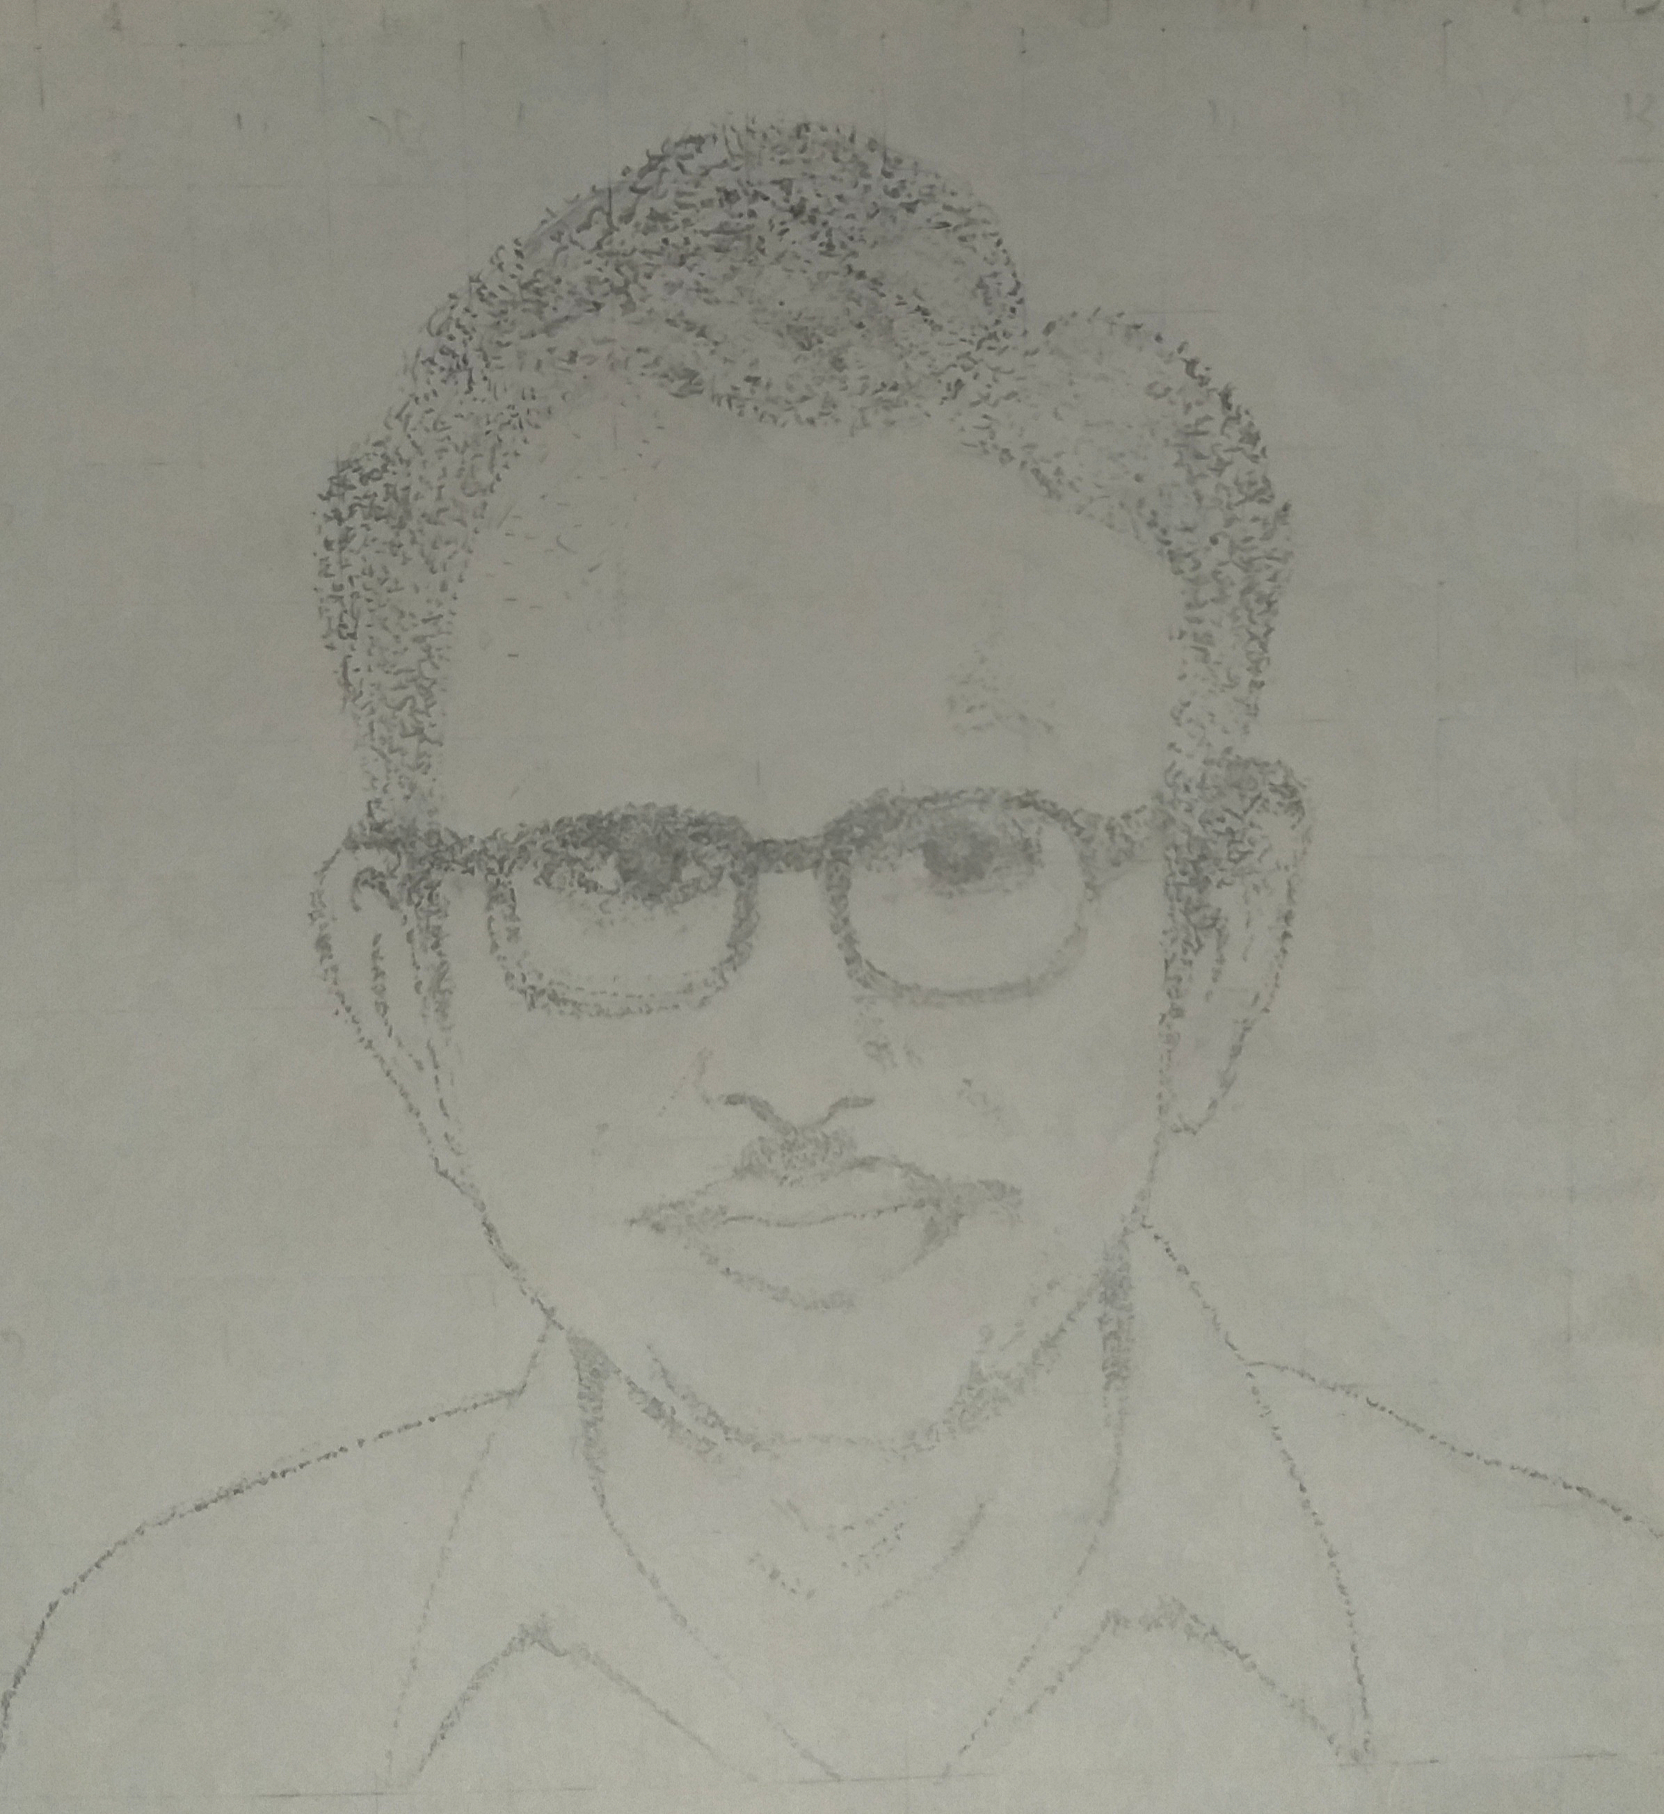
\includegraphics[scale=.25]{figures/chap15-fig1.eps}
}
\end{figure}


Dr. K S Mallesh, Former Professor, DoS in Physics, University of Mysore, Manasagangotri, Mysuru 570 006, email: ksmallesh@gmail.com, Phone no. 9900598270

%~ \begin{tabular}{V{2.5}cp{14.2cm}V{2.5}}
%~ \clineB{1-2}{2.5}
 %~ &\\
%~ \raisebox{-4cm}{\includegraphics{src/figures/authors/ Prof_K_S_Mallesh.jpg}} & 

%~ \centerline{\large\bf K.S.Mallesh}

%~ \bigskip
%~ Dr. K.S.Mallesh obtained M. Sc. degree in 1979 and Ph.D. in 1990 from the University of Mysore.  He worked for Ph.D.  under the guidance of Prof. G.Ramachandran.  He served as a Lecturer in Yuvaraja’s College from 1982 to 1994. Later, he joined the Department of Studies in Physics, University of Mysore, in 1994 and taught there till his retirement in 2019.  He worked closely with GR during this period.  Currently he is leading an active retired life in Mysuru.\\
%~ &\\ 
%~ \clineB{1-2}{2.5}
%~ \end{tabular}
